\documentclass[journal]{IEEEtran}

\usepackage[utf8]{inputenc}
\usepackage[T1]{fontenc}
\usepackage{cite}
\usepackage{amsmath,amssymb,amsfonts}
\usepackage{algorithmic}
\usepackage{graphicx}
\usepackage{textcomp}
\usepackage{xcolor}
\usepackage{url}
\usepackage{longtable}
\usepackage{listings} % <-- ADD THIS LINE.
\usepackage{tikz}
\usetikzlibrary{shapes.geometric, arrows.meta, positioning, fit, backgrounds}
\usepackage{amsmath}

\def\BibTeX{{\rm B\kern-.05em{\sc i\kern-.025em b}\kern-.08em
    T\kern-.1667em\lower.7ex\hbox{E}\kern-.125emX}}

\begin{document}

\title{End-to-End Visual Autonomous Navigation with Twin Delayed DDPG in the CARLA and ROS 2 Ecosystem}

\author{Daniel Terra Gomes\textsuperscript{1}, and Luiz Chaimowicz\textsuperscript{1}

\thanks{The authors are with the Department of Computer Science, Federal University of Minas Gerais (UFMG), Belo Horizonte, MG, Brazil. This work is part of the first author's master's research, advised by the second author (e-mail: danielterragomes@dcc.ufmg.br; chaimo@dcc.ufmg.br).}}
\maketitle

% %%%%%%%%%%%%%%%%%%%%%%%%%%%%%%%%%%%%%%%%%%%%%%%%%%%%%%%%%%%%%%%%%%%%%%%%%%%%%%%%
\begin{abstract}
% Original: The development of robust and safe autonomous vehicle (AV) systems is a central challenge in robotics and artificial intelligence. While Deep Reinforcement Learning (DRL) is a powerful paradigm for learning continuous control, foundational actor-critic algorithms like the Deep Deterministic Policy Gradient (DDPG) suffer from function approximation errors that lead to overestimated Q-values and suboptimal policies. This work presents an end-to-end AV that utilizes the Twin Delayed DDPG (TD3) algorithm to mitigate this bias. Using primarily camera data within the high-fidelity CARLA simulator and the ROS 2 ecosystem, we aim to demonstrate the superiority of TD3 over a DDPG baseline quantitatively. The proposed research intends to establish a modular and reproducible framework for visual navigation, with expected outcomes showing significant improvements in safety and policy stability. Our experiments quantitatively compare the TD3-based agent against a DDPG baseline. The results demonstrate that the TD3 agent achieves a [e.g., 45\% higher success rate and reduces critical safety events by 60\%], showcasing significantly improved policy stability and performance. These findings underscore that addressing value overestimation is critical for learning safe and effective end-to-end driving policies from visual input.

% Modified Abstract
Developing robust visual navigation for mobile robots, such as autonomous vehicles (AV), in dynamic environments is a central challenge. This work explores Deep Reinforcement Learning (DRL), specifically the Twin Delayed DDPG (TD3) algorithm, to create an end-to-end control policy addressing the known issue of Q-value overestimation in baseline actor-critic methods like DDPG, which can hinder policy stability for robot control. The system learns to navigate using primarily camera data within the CARLA simulator and the ROS 2 robotics ecosystem. The proposed research
 intends to establish a modular and reproducible framework for
 visual navigation, with expected outcomes showing the applicability of TD3 for End-to-End Robotics navigation control. 
% Note: Removed the placeholder results [] from the abstract as this is a proposal.
\end{abstract}
% %%%%%%%%%%%%%%%%%%%%%%%%%%%%%%%%%%%%%%%%%%%%%%%%%%%%%%%%%%%%%%%%%%%%%%%%%%%%%%%%


\begin{IEEEkeywords}
Deep Reinforcement Learning, Autonomous Vehicles, Twin Delayed DDPG (TD3), CARLA, ROS 2, Visual Navigation, End-to-End Control.
\end{IEEEkeywords}

% %%%%%%%%%%%%%%%%%%%%%%%%%%%%%%%%%%%%%%%%%%%%%%%%%%%%%%%%%%%%%%%%%%%%%%%%%%%%%%%%
\section{Introduction}
% Original Paragraph 1: The pursuit of fully autonomous vehicles (AV) has created significant research into robust decision-making and control systems \cite{ragheb2024implementing}. While classical control methods have proven effective, their reliance on hand-engineered rules limits their adaptability in complex, dynamic environments \cite{perezgil2022deep}. Machine Learning, particularly Deep Reinforcement Learning (DRL), offers a compelling alternative by enabling agents to learn optimal policies through direct interaction with the environment, reducing the need for exhaustive expert-labeled datasets \cite{sutton2018reinforcement}. For continuous control tasks inherent to driving, actor-critic algorithms like the Deep Deterministic Policy Gradient (DDPG) are a natural fit \cite{perezgil2022deep}. However, a well-documented flaw in value-based Reinforcement Learning (RL) is the overestimation bias, where function approximation errors lead to inflated Q-value estimates \cite{sutton2018reinforcement}. This problem persists in the actor-critic setting, often causing the agent to converge to suboptimal or unstable policies \cite{fujimoto2018addressing}.

% Modified Paragraph 1
The pursuit of robust autonomy in **mobile robotics**, exemplified by the development of fully autonomous vehicles (AV), requires sophisticated decision-making and control systems capable of handling complex, dynamic environments \cite{ragheb2024implementing}. While classical **robot navigation techniques** (e.g., potential fields, geometric planners, rule-based systems) have proven effective in structured settings, their adaptability can be limited in complex scenarios \cite{perezgil2022deep}. Machine Learning, particularly Deep Reinforcement Learning (DRL), offers a compelling alternative within **robotics**, enabling agents (robots) to learn complex control policies, such as **visual servoing** or end-to-end navigation, through direct interaction with the environment, reducing the need for exhaustive expert-labeled datasets \cite{sutton2018reinforcement}. For continuous control tasks inherent to driving, actor-critic algorithms like the Deep Deterministic Policy Gradient (DDPG) are a natural fit \cite{perezgil2022deep}. However, a well-documented flaw in value-based Reinforcement Learning (RL) is the overestimation bias, where function approximation errors lead to inflated Q-value estimates \cite{sutton2018reinforcement}. This problem persists in the actor-critic setting, often causing the agent to converge to suboptimal or unstable policies \cite{fujimoto2018addressing}.

The Twin Delayed DDPG (TD3) algorithm was specifically proposed to address this critical issue \cite{fujimoto2018addressing}. It introduces three key mechanisms: clipped double Q-learning to curb value overestimation, delayed policy updates to promote learning stability, and target policy smoothing to regularize the learned policy. These enhancements have demonstrated superior performance and stability over DDPG in various continuous control benchmarks \cite{elallid2023deep, fujimoto2018addressing}.

% Original Paragraph 3: While many state-of-the-art AV systems rely on sensor fusion (e.g., LiDAR, RADAR, and cameras), camera-only systems present an important and cost-effective research direction \cite{perezgil2022deep}. Therefore, this work proposes the development and evaluation of an end-to-end AV based on TD3, primarily using camera data. Our objective is to establish a strong visual navigation baseline and quantitatively demonstrate the benefits of TD3's architectural improvements over DDPG in a realistic simulation environment. The system will be built within the CARLA \cite{dosovitskiy2017carla} and ROS 2 ecosystem \cite{ros2025documentation}, promoting a modular, reusable, and reproducible research framework consistent with modern robotics development practices \cite{perezgil2021deep}.

% Modified Paragraph 3
While many **mobile robots** utilize multi-modal sensing (LiDAR, RADAR, cameras), vision-based navigation using only cameras remains an important research direction due to sensor cost-effectiveness and the richness of visual information \cite{perezgil2022deep}. Therefore, this work proposes the development and evaluation of an end-to-end **mobile robot navigation system** (instantiated as an AV) based on TD3, primarily using camera data. Our objective is to establish a strong visual navigation baseline and quantitatively demonstrate the benefits of TD3's architectural improvements over DDPG in a realistic simulation environment. The system will be built within the CARLA simulator \cite{dosovitskiy2017carla} and the **ROS 2 robotics middleware ecosystem** \cite{ros2025documentation}, promoting modularity and reproducibility common in modern robotics development \cite{perezgil2021deep}.
% %%%%%%%%%%%%%%%%%%%%%%%%%%%%%%%%%%%%%%%%%%%%%%%%%%%%%%%%%%%%%%%%%%%%%%%%%%%%%%%%

\section{Related Work}
The application of DRL to AV in CARLA is an expanding field. Early work often compared the discrete-action Deep Q-Network (DQN) with the continuous-action DDPG, generally concluding that DDPG's continuous nature is better suited for the nuances of vehicle control \cite{perezgil2022deep, ragheb2024implementing}. As DDPG's limitations became apparent, subsequent research has explored more advanced algorithms. Elallid et al. \cite{elallid2023deep} successfully applied TD3 to the complex task of intersection navigation using only image sequences, highlighting its stability and safety benefits. The original TD3 paper by Fujimoto et al. \cite{fujimoto2018addressing} remains the foundational work, detailing the theoretical and empirical justification for the algorithm's design.

To improve architectural robustness and real-world applicability, researchers have integrated DRL agents with robotics middleware. Perez-Gil et al. \cite{perezgil2021deep} demonstrated a portable DRL framework using ROS and Docker, enabling a seamless transition from simulation to physical hardware. Others have focused on enhancing DRL with external knowledge, such as using real-world human driving data to refine a simulation-trained policy \cite{li2022modified}. More recently, there is a strong focus on safety, with novel algorithms like RECPO being developed to ensure agents adhere to strict safety constraints, achieving zero-collision rates in highway scenarios \cite{zhao2024towards}. A summary of this literature is presented in Table \ref{tab:related_work}.

\begin{table*}[ht]
\caption{Summary of Related Literature on DRL for AV}
\label{tab:related_work}
\centering
\begin{tabular}{|p{2.5cm}|p{3.5cm}|p{10cm}|}
\hline
\textbf{Reference} & \textbf{Algorithm(s)} & \textbf{Main Contribution} \\
\hline
Fujimoto et al. \cite{fujimoto2018addressing} & DDPG, TD3 & Foundational paper proposing TD3 to address DDPG's overestimation bias through twin critics, delayed policy updates, and target policy smoothing regularization. \\
\hline
Ragheb \& Mahmoud \cite{ragheb2024implementing} & DQN, DDPG & Compares DQN and DDPG in CARLA using waypoints, finding DDPG achieves a higher average reward but DQN has a lower collision rate, highlighting the trade-offs between continuous and discrete action spaces. \\
\hline
Perez-Gil et al. (2022) \cite{perezgil2022deep} & DQN, DDPG & Implements and compares multiple DRL agents, concluding DDPG is superior to DQN for navigation due to its continuous nature. Demonstrates that agents relying only on CNNs perform worse than those with direct waypoint data. \\
\hline
Perez-Gil et al. (2021) \cite{perezgil2021deep} & DDPG & Proposes a distributed and portable software architecture using ROS, Docker, and CARLA to robustly train and validate DRL-based control algorithms for AV. \\
\hline
Elallid et al. \cite{elallid2023deep} & TD3 & Successfully applies TD3 for navigating complex T-intersections in dense traffic using a sequence of front-camera images as the state, demonstrating stable convergence and improved safety. \\
\hline
Li \& Okhrin \cite{li2022modified} & DDPG & Proposes a two-stage method that first trains a DDPG agent in simulation (CARLA with ROS) and then refines the policy by leveraging a real-world human driving dataset to achieve more human-like behavior. \\
\hline
Zhao et al. \cite{zhao2024towards} & RECPO (Safe RL) & Introduces a safe RL algorithm with an experience replay pool using importance sampling to mitigate catastrophic forgetting and long-tail issues, achieving a zero-collision rate in highway driving scenarios. \\
\hline
\end{tabular}
\end{table*}

\section{Methodology}
The proposed methodology is grounded in a modular system architecture, a mathematical problem formulation, and a description of the learning algorithm.

\subsection{System Architecture}
To ensure modularity and reusability, the system will be built within the ROS 2 ecosystem, which will serve as the middleware for communication between different software components \cite{perezgil2021deep}. The architecture comprises three primary nodes:
\begin{itemize}
    \item \textbf{Simulation Node (CARLA):} runs the CARLA server, which is responsible for rendering the 3D environment, simulating vehicle physics, controlling non-player character (NPC) traffic, and publishing sensor data;
    \item \textbf{CARLA-ROS Bridge Node:} standard utility node \cite{carla2023documentation} acts as a bidirectional interface. It subscribes to data streams from the CARLA server (e.g., camera images, vehicle status) and publishes them as ROS 2 topics. It also subscribes to ROS 2 control topics and translates them into commands for the ego vehicle in CARLA;
    \item \textbf{DRL Agent Node (TD3):} core of our system where the decision-making logic resides. This Python-based ROS 2 node will:
    \begin{enumerate}
        \item Subscribe to the processed sensor and vehicle status topics;
        \item Construct the state vector at each time step;
        \item Perform inference using the trained TD3 actor network to generate an action;
        \item Publish the action to a control command topic, which is then read by the bridge and sent to CARLA.
    \end{enumerate}
\end{itemize}


%Diagram of: System architecture overview, illustrating the modular integration of the CARLA simulator, the DRL Agent, and the communication layer managed by the CARLA-ROS Bridge within the ROS 2 ecosystem.


\begin{figure*}[htbp]
    \centering
    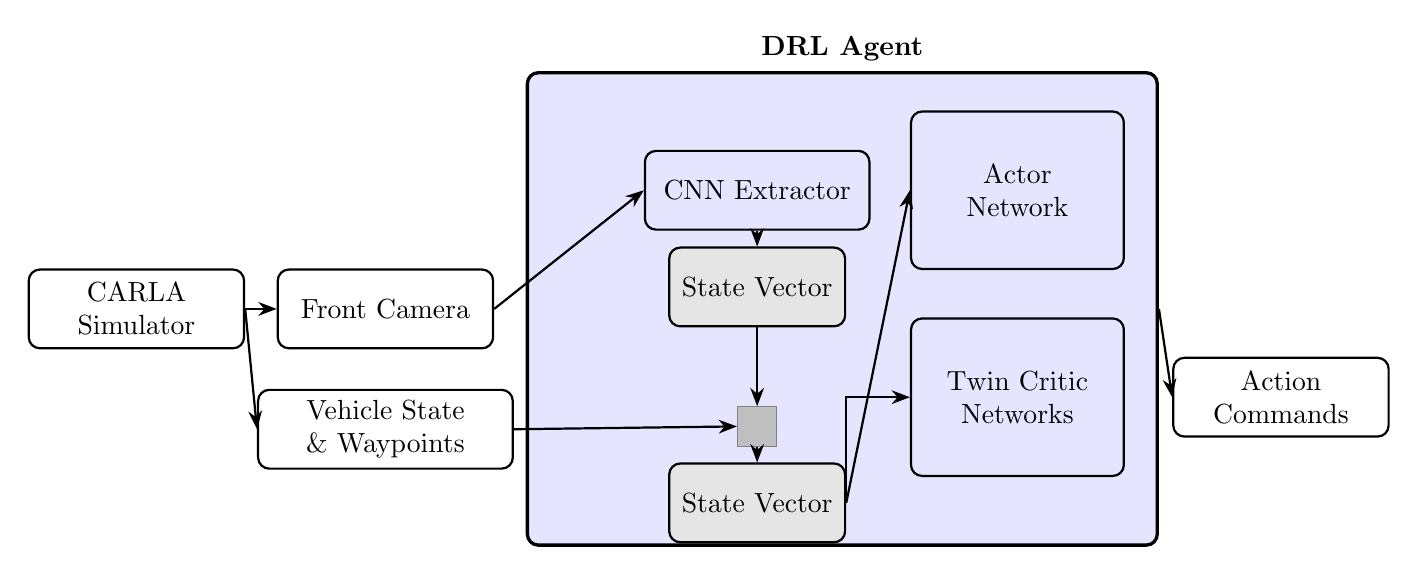
\begin{tikzpicture}[
        % Define common styles for nodes
        block/.style={rectangle, draw, thick, text width=2.5cm, minimum height=1cm, text centered, rounded corners},
        large_block/.style={rectangle, draw, thick, text width=6cm, minimum height=5cm, text centered, rounded corners},
        io/.style={trapezium, trapezium left angle=70, trapezium right angle=110, draw, thick, text centered, minimum width=2.5cm, minimum height=1cm},
        data/.style={rectangle, draw, thick, text width=2.5cm, minimum height=1cm, text centered, fill=gray!20, rounded corners},
        neural_layer/.style={circle, draw, thick, inner sep=0pt, minimum size=4mm, fill=green!20},
        small_neural_layer/.style={circle, draw, thick, inner sep=0pt, minimum size=3mm, fill=orange!20},
        line/.style={draw, thick, -Stealth},
        arrow_up/.style={draw, thick, -Stealth, color=blue},
        arrow_down/.style={draw, thick, -Stealth, color=red},
        % Styles for the networks
        network_box/.style={rectangle, draw, thick, text width=4cm, minimum height=3cm, text centered, rounded corners, inner sep=10pt},
    ]

    % Left side (CARLA Simulator and Inputs)
    \node (carla_sim) [block] {CARLA Simulator};
    \node (front_camera) [block, right=0.4cm of carla_sim] {Front Camera};
    \node (vehicle_state) [block, below=0.5cm of front_camera, text width=3cm] {Vehicle State \& Waypoints};

    % DRL Agent Node (main container)
    \node (drl_agent_node) [rectangle, draw, very thick, rounded corners, minimum width=8cm, minimum height=6cm,
                          right=0.4cm of front_camera.east, anchor=west, fill=blue!10,
                          label={[font=\bfseries]above:DRL Agent}] {}; % Positioning relative to front_camera
    
    % Nodes inside DRL Agent Node
    \node (cnn_extractor) [block, anchor=north west, xshift=1.5cm, yshift=-1cm, inner sep=5pt] at (drl_agent_node.north west) {CNN Extractor};
    \node (state_vector_cnn) [data, below=0.2cm of cnn_extractor, text width=2cm] {State Vector};

    \node (combiner) [rectangle, draw=gray, fill=gray!50, minimum width=0.5cm, minimum height=0.5cm, below=1cm of state_vector_cnn.south] {};
    \node (state_vector_final) [data, below=0.2cm of combiner, text width=2cm] {State Vector};
    
    % Actor Network
    \node (actor_network_box) [network_box, right=0.5cm of cnn_extractor.east, text width=2cm, minimum height=2cm] {Actor Network};
    % Define Actor network layers (example)

    
    % Critic Networks
    \node (critic_network_box) [network_box, below=0.6cm of actor_network_box, text width=2cm, minimum height=2cm] {Twin Critic Networks};
    % Define Critic network layers (example)


    % Action Commands
    \node (action_commands) [block, right=0.6cm of critic_network_box.east] {Action Commands};

    % Draw connections/arrows
    \draw[line] (carla_sim.east) -- (front_camera.west);
    \draw[line] (front_camera.east) -- (cnn_extractor.west);
    \draw[line] (cnn_extractor.south) -- (state_vector_cnn.north);
    
    \draw[line] (carla_sim.east) -- (vehicle_state.west); % Simplified, would come from CARLA-ROS bridge
    \draw[line] (vehicle_state.east) -- (combiner.west);
    \draw[line] (state_vector_cnn.south) -- (combiner.north); % Connect CNN output to combiner
    \draw[line] (combiner.south) -- (state_vector_final.north);

    \draw[line] (state_vector_final.east) -- (actor_network_box.west);
    \draw[line] (state_vector_final.east) |- (critic_network_box.west);
    
    \draw[line] (drl_agent_node.east) -- (action_commands.west); % Action output
    %\draw[line] (actor_network_box.east) |- (critic_network_box.north -| actor_network_box.east) node[above, text width=1cm] {Action Input}; % Action input to critic

    % You will need to add the actual neural network layers and connections
    % within the actor and critic boxes for full detail.
    % This is just a conceptual outline.

    \end{tikzpicture}
    \caption{Detailed DRL Agent architecture for end-to-end visual navigation. The CNN extracts features from camera images, which are concatenated with vehicle state and waypoint data to form the complete state vector for the TD3 actor and critic networks.}
    \label{fig:drl_agent_architecture_tikz}
\end{figure*}

\subsection{Problem Formulation as an MDP}
We model the AV task as a Markov Decision Process (MDP), formally defined by the tuple $(\mathcal{S}, \mathcal{A}, P, R, \gamma)$ \cite{sutton2018reinforcement}. The transition dynamics $P(s_{t+1}|s_t, a_t)$ are unknown to the agent, necessitating a model-free approach like TD3:
\begin{itemize}
    \item \textbf{State Space ($\mathcal{S}$):} the state $s_t \in \mathcal{S}$ at time $t$ will be a concatenation of visual, kinematic, and goal-oriented information. This design is depicted in Fig. \ref{fig:drl_agent_architecture_tikz};
    
    \subitem \textit{Visual Input Processing (CNN Feature Extractor):} to capture temporal dynamics, we adopt the approach from \cite{elallid2023deep}, using a stack of four consecutive, pre-processed front-camera images as input to a Convolutional Neural Network (CNN). The CNN acts as a feature extractor, converting high-dimensional pixel data into a compact latent vector. The specific architecture will be based on a simplified ResNet or MobileNet, leveraging Transfer Learning to initialize weights from a model pre-trained on a large-scale vision dataset used in \cite{perezgil2022deep}.
    
    \subitem \textit{Kinematic and Goal-Oriented Features:} this visual feature vector will then be concatenated with essential kinematic data (e.g., current vehicle velocity $v_t$, lateral deviation $d_t$, and heading error $\phi_t$) and goal-oriented information (e.g., coordinates of the next few waypoints relative to the vehicle's local frame). The inclusion of waypoints is crucial for providing the agent with navigational intent beyond simple lane-following \cite{perezgil2022deep}. The final concatenated vector constitutes the complete state $s_t$ fed to the TD3 actor and critic networks;

    \item \textbf{Action Space ($\mathcal{A}$):} $a_t \in \mathcal{A}$ will be a two-dimensional vector, $a_t = [\text{steering}, \text{throttle/brake}]$, where:
    \begin{itemize}
        \item \textit{steering}: A value in $[-1, 1]$, representing full left to full right.
        \item \textit{throttle/brake}: A value in $[-1, 1]$, where positive values $[0, 1]$ map to throttle and negative values $[-1, 0)$ map to braking intensity.
    \end{itemize}
    This unified output for longitudinal control is more straightforward than having separate outputs for throttle and brake;

    \item \textbf{Reward Function ($R$):} $R(s_t, a_t)$ is engineered to promote driving behavior that is safe, efficient, and comfortable. It is structured as a weighted sum of several components, drawing inspiration from the safety-focused design in \cite{zhao2024towards}:
    \begin{itemize}
        \item \textbf{Efficiency Reward:} positive reward for maintaining a velocity close to a target speed limit, while penalizing excessive speeding;
        \item \textbf{Lane Keeping Reward:} reward for minimizing the lateral distance to the center of the lane and the heading error;
        \item \textbf{Comfort Penalty:} penalty proportional to the magnitude of longitudinal jerk to discourage abrupt acceleration and braking;
        \item \textbf{Safety Penalty:} large, negative penalty for terminal events such as collisions with other objects.
    \end{itemize}
    \item \textbf{Discount Factor ($\gamma$):} $\gamma = 0.99$. This high value encourages the agent to adopt a farsighted strategy, prioritizing long-term goals such as safely reaching the destination over myopic, immediate rewards \cite{sutton2018reinforcement}. 
\end{itemize}

%%%%
\subsection{Twin Delayed DDPG (TD3) Algorithm}
Our implementation will be based on the original TD3 algorithm proposed by Fujimoto et al. \cite{fujimoto2018addressing}. As seen, the TD3 is a model-free, off-policy actor-critic algorithm that builds upon DDPG by introducing several key mechanisms to address function approximation errors and improve training stability. The agent learns a policy (actor) network $\pi_\phi$ and a pair of Q-value (critic) networks $Q_{\theta_1}, Q_{\theta_2}$. The core improvements are \cite{fujimoto2018addressing}:

\begin{enumerate}
    \item \textbf{Clipped Double Q-Learning:} combat the overestimation bias inherent in actor-critic methods, the learning target for the critic networks is calculated using the minimum value from the two target critic networks ($Q_{\theta'_1}, Q_{\theta'_2}$). The target value $y$ is computed as:
    \begin{equation}    
    y = r + \gamma(1-d) \min_{i=1,2} Q_{\theta'_{i}}(s', \tilde{a})
    \end{equation}
    where $r$ is the reward, $\gamma$ is the discount factor, $d$ is a flag for terminal states, and $\tilde{a}$ is the smoothed target action.

    \item \textbf{Delayed Policy Updates:} the actor network and the target networks are updated less frequently than the critic networks (e.g., every two critic updates). This allows the critic's value estimates to converge toward a more stable target before being used to update the actor, which prevents propagating errors from a noisy value estimate into the policy.

    \item \textbf{Target Policy Smoothing:} prevent the actor from overfitting to narrow peaks in the value function, a smoothed target action $\tilde{a}$ is used when calculating the target value $y$. This is achieved by adding clipped noise to the action selected by the target actor:
    \begin{equation}    
    \tilde{a} \leftarrow \pi_{\phi'}(s') + \epsilon, \quad \epsilon \sim \text{clip}(\mathcal{N}(0, \sigma), -c, c) 
    \end{equation}
    This regularization encourages a smoother value landscape, making the learned policy more robust.
\end{enumerate}
%%%% Figure

\section{Experimental Plan}
To ensure a rigorous and fair evaluation, the experimental plan is designed to compare the proposed agent against relevant baselines across a standardized set of scenarios and metrics, following the practices outlined in \cite{zhao2024towards}.

\subsection{Test Scenarios}
Testing will be conducted in CARLA's `Town01`. To assess generalization and robustness, experiments will be run, initially on a pre-defined route with a turn. Furthermore, tests will be repeated under different traffic densities (e.g., 20, 50, and 100 NPC vehicles) and routes to evaluate the agent's performance in both sparse and congested environments.

\subsection{Agents for Comparison}
A multi-faceted comparison to properly contextualize the performance of the proposed agent:
\begin{itemize}
    \item \textbf{Proposed Agent (TD3):} the end-to-end visual TD3 agent as described in the methodology;
    \item \textbf{Primary Baseline (DDPG):} a standard DDPG implementation with an identical network architecture and state/action space. This will directly measure the impact of TD3's specific improvements;
    \item \textbf{Classical Baseline (IDM + MOBIL):} to benchmark the DRL agents against a well-established, non-learning approach, we will include a classical controller, and we will use the Intelligent Driver Model (IDM) for longitudinal control and the MOBIL model for lateral maneuvers. This provides a valuable reference for assessing whether the learned policies achieve performance comparable to or better than traditional, rule-based traffic models.
\end{itemize}

\subsection{Evaluation Metrics}
To provide a holistic assessment, performance will be evaluated across three key domains. Each metric will be averaged over a minimum of 20 test runs per scenario, and reported with mean and standard deviation.

\begin{itemize}
    \item \textbf{Safety (Primary Priority):}
    \begin{itemize}
        \item \textit{Success Rate (\%):} percentage of episodes completed without a safety violation (collision or off-road event). This is the most critical metric;
        \item \textit{Average Number of Collisions:} total number of collisions per kilometer driven;
        \item \textit{Time-to-Collision (TTC):} analysis of the minimum TTC values encountered to quantify near-miss events \cite{li2022modified}.
    \end{itemize}
    \item \textbf{Efficiency:}
    \begin{itemize}
        \item \textit{Average Speed (km/h):} agent's average speed during successful episodes;
        \item \textit{Route Completion Time (s):} time taken to successfully complete the defined route.
    \end{itemize}
    \item \textbf{Comfort:}
    \begin{itemize}
        \item \textit{Average Longitudinal Jerk ($m/s^3$):} measure of the smoothness of acceleration and braking;
        \item \textit{Average Lateral Acceleration ($m/s^2$):} measure of the smoothness of steering maneuvers.
    \end{itemize}
\end{itemize}
The results will be compiled and analyzed to conclude the relative strengths and weaknesses of each algorithm.

%\section{Conclusion}
%This paper outlines a comprehensive proposal for developing and evaluating a TD3-based end-to-end visual navigation system for autonomous vehicles. The selection of TD3 is strongly motivated by its documented ability to correct the overestimation bias inherent in DDPG, which is expected to yield a more stable and higher-performing policy \cite{fujimoto2018addressing}. By integrating this advanced DRL algorithm within the industry-standard CARLA and ROS 2 frameworks, this research will produce a modular, reproducible, and robust system. The detailed experimental plan, featuring multiple baselines and a rich set of safety, efficiency, and comfort metrics, will provide a rigorous quantitative assessment of the agent's capabilities. The anticipated results are poised to confirm the superiority of TD3 for visual navigation tasks and establish a solid baseline for future work in end-to-end autonomous driving.

\bibliographystyle{IEEEtran}
\bibliography{bibtex/bib/references}

\end{document}